\documentclass[a5paper,headsepline,titlepage,11pt,nnormalheadings,DIVcalc]{scrbook}
\usepackage[a5paper,backref]{hyperref}
\usepackage[papersize={148.5mm,215mm},twoside,bindingoffset=0.5cm,hmargin={2cm,2cm},
				vmargin={2cm,2cm},footskip=1.1cm,driver=dvipdfm]{geometry}
\usepackage{palatino}
\usepackage{graphicx}
\usepackage{wrapfig}
\usepackage[bahasa]{babel}
\usepackage{fancyhdr}
\usepackage{longtable}
\usepackage{hhline,multirow}
\usepackage{pst-node}

\renewcommand{\footrulewidth}{0.5pt}
\lhead[\fancyplain{}{\thepage}]%
      {\fancyplain{}{~}}
\rhead[\fancyplain{}{~}]%
      {\fancyplain{}{\thepage}}
\pagestyle{fancy}
\lfoot[\emph{Doa 40 hari \namaalm}]{}
\rfoot[]{\emph{Lingkungan St Petrus Maguwo}}
\cfoot{}

\newcommand{\BU}[1]{\begin{itemize} \item[U:] #1 \end{itemize}}
\newcommand{\BI}[1]{\begin{itemize} \item[I:] #1 \end{itemize}}
\newcommand{\BP}[1]{\begin{itemize} \item[P:] #1 \end{itemize}}
\newcommand{\BPP}[1]{\begin{itemize} \item[Bpk:] #1 \end{itemize}}
\newcommand{\BPW}[1]{\begin{itemize} \item[Ibu:] #1 \end{itemize}}
\newcommand{\namaalm}{Bapak Vincentius Muharto~}
\newcommand{\namaromo}{~}
\title{Ibadat/Doa untuk Arwah}
\author{}
\date{2011}
\hyphenation{sa-u-da-ra-ku}
\hyphenation{ke-ri-ngat}
\hyphenation{je-ri-tan}
\hyphenation{hu-bung-an}
\hyphenation{me-nya-dari}
\hyphenation{Eng-kau}
\hyphenation{ke-sa-lah-an}
\hyphenation{ba-gai-ma-na}
\hyphenation{Tu-han}
\hyphenation{di-per-ca-ya-kan}
\hyphenation{men-ja-uh-kan}
\hyphenation{bu-kan-lah}
\hyphenation{per-sa-tu-kan-lah}
\hyphenation{ma-khluk}
\hyphenation{Sem-buh-kan-lah}
\hyphenation{ja-lan}
\hyphenation{mem-bu-tuh-kan}
\hyphenation{be-ri-kan-lah}
\hyphenation{me-ra-sa-kan}
\hyphenation{te-man-ilah}
\hyphenation{mem-bi-ngung-kan}
\hyphenation{di-ka-gum-i}
\hyphenation{ta-ngis-an-Mu}
\hyphenation{mi-lik-ilah}

\renewcommand*\thesection{\arabic{section}.}
\setlength{\parindent}{0mm} 

\begin{document}
\thispagestyle{empty}
%\maketitle
%\newsavebox\IBox
%\sbox\IBox{\includegraphics[scale=0.4]{Saint-Peter-Apostle-e.eps}}

\psset{unit=1in}
\begin{pspicture}(4in,6.0in)
% set up the fonts we use
\DeclareFixedFont{\PT}{T1}{ppl}{b}{it}{0.4in}
\DeclareFixedFont{\PTsmall}{T1}{ppl}{b}{it}{0.3in}
\DeclareFixedFont{\PTsmallest}{T1}{ppl}{b}{it}{0.2in}
\DeclareFixedFont{\PTtext}{T1}{ppl}{b}{it}{11pt}
\DeclareFixedFont{\Logo}{T1}{pbk}{m}{n}{0.2in}
% place the front cover picture
%\rput[cb](2.3,2.5){\usebox\IBox}
% put the text on the front cover
\rput[cb](2.5,5.3){\PTsmall {Ibadat/Doa Arwah 40 hari untuk}}
\rput[cb](2.5,4.8){\PTsmall {\namaalm}}
\rput[cb](2.5,1.1){\PTsmall {8 November 2011}}
\rput[cb](2.5,0.6){\PTsmallest {Wilayah Yohanes de Britto}}
\rput[cb](2.5,0.3){\PTsmallest {Stasi Maguwo}}
\rput[cb](2.5,0.0){\PTsmallest {Paroki Marganingsih Kalasan }}

%\rput[cb](3,-1){\PTsmallest {\namagereja}} 

\end{pspicture}
%\tableofcontents 
\newpage
\thispagestyle{empty}
{~}
\newpage
\setlength{\parskip}{2mm}

\section*{RITUS PEMBUKA}
\subsection*{LAGU PEMBUKA}

\subsection*{SALAM PEMBUKAAN}
\BP{Atas nama Bapa Putera dan Roh Kudus} 
\BU{Amin}
\BP{Semoga damai sejahtera Tuhan kita Yesus Kristus, cinta kasih Allah Bapa dan persekutuan Roh Kudus, selalu beserta kita.}
\BU{Sekarang dan selama-lamanya}

\subsection*{PENGANTAR}
\BP{Bapak, Ibu, Saudara Saudari yang terkasih dalam Kristus, 40 hari yang lalu keluarga ini mengalami duka yang mendalam. Kalau ditanya mengapa berduka? Jawabanya adalah karena pada waktu itu \namaalm telah dipanggil Tuhan. Mungkin kita bisa ikut merasakan perasaan / suasana hati dari keluarga yang ditinggalkan pada waktu itu. Sebagai ungkapan cinta keluarga ini terhadap almarhumah \namaalm kita semua diundang untuk bersama-sama mendukung dengan doa-doa supaya arwah dari \namaalm segera dapat ikut bangkit mulia bersama Kristus di dalam kerajaan surga.}

\emph{Hening sejenak \dots}
  
\subsection*{PERNYATAAN TOBAT}
\BP{Saudara-saudari yang seiman dalam Kristus, marilah kita membuat diri pantas berada di depan hadirat Allah, dengan membersihkan diri kita dari dosa dan kesalahan yang lalu, dengan bertobat dan mohon ampun kepada Allah kita.}

\BP{Saya mengaku \dots}

\BP{Semoga Allah yang mahakuasa mengasihani kita, 
mengampuni dosa kita dan mengantar kita ke dalam hidup 
yang kekal.}

\BU{Amin}

\subsection*{Tuhan Kasihanilah Kami}

\subsection*{Doa Pembuka}
\BP{Marilah Berdoa 

Allah Bapa yang mahamurah, Engkau telah menyerahkan 
Yesus, Putra-Mu kepada kematian, semua ini harus terjadi 
untuk melepaskan kami dari segala kuasa kegelapan dan 
dosa. Ya Bapa, anugerahkanlah hidup kekal kepada 
\namaalm yang telah menghadap 
kehadiratMu 40 hari yang lalu. Ya Bapa, ampunilah 
segala dosa dan kesalahannya dan bukalah pintu 
kehidupan kekal baginya. Terimalah saudara kami 
tercinta ini kedalam keluarga kudusMu di tahta surgawi. }

\BU{Amin} 
 
\section*{IBADAT SABDA}
\BP{Saudara-saudari terkasih marilah kita mempersiapkan hati 
dan budi untuk mendengarkan sabda Tuhan.} 

\subsection*{BACAAN PERTAMA}

\BP{Pembacaan dari 1 Kor 15:12-18 

Saudara-saudara bilamana kami beritakan, bahwa Kristus dibangkitkan dari antara orang mati, bagaimana mungkin ada di antara kamu yang mengatakan, bahwa tidak ada kebangkitan orang mati?
Kalau tidak ada kebangkitan orang mati, maka Kristus juga tidak dibangkitkan.

Tetapi andaikata Kristus tidak dibangkitkan, maka sia-sialah pemberitaan kami dan sia-sialah juga kepercayaan kamu.
Lebih dari pada itu kami ternyata berdusta terhadap Allah, karena tentang Dia kami katakan, bahwa Ia telah membangkitkan Kristus?padahal Ia tidak membangkitkan-Nya, kalau andaikata benar, bahwa orang mati tidak dibangkitkan.

Sebab jika benar orang mati tidak dibangkitkan, maka Kristus juga tidak dibangkitkan.
Dan jika Kristus tidak dibangkitkan, maka sia-sialah kepercayaan kamu dan kamu masih hidup dalam dosamu.
Demikianlah binasa juga orang-orang yang mati dalam Kristus. 

Demikianlah sabda Tuhan }

\BU{Syukur kepada Allah} 

\subsection*{LAGU TANGGAPAN} 

\subsection*{Bacaan Injil} 

\BP{Tuhan beserta kita} 
\BU{Sekarang dan selama-lamanya} 
\BP{Inilah Injil Yesus Kristus menurut Yohanes (6:37-40) 

Semua yang diberikan Bapa kepada-Ku akan datang kepada-Ku, dan barangsiapa datang kepada-Ku, ia tidak akan Kubuang.
Sebab Aku telah turun dari sorga bukan untuk melakukan kehendak-Ku, tetapi untuk melakukan kehendak Dia yang telah mengutus Aku.

Dan Inilah kehendak Dia yang telah mengutus Aku, yaitu supaya dari semua yang telah diberikan-Nya kepada-Ku jangan ada yang hilang, tetapi supaya Kubangkitkan pada akhir zaman.
Sebab inilah kehendak Bapa-Ku, yaitu supaya setiap orang, yang melihat Anak dan yang percaya kepada-Nya beroleh hidup yang kekal, dan supaya Aku membangkitkannya pada akhir zaman.

Demikianlah Injil Tuhan} 

\BU{Terpujilah Kristus}

\subsection*{HOMILI}

``Semua yang telah diberikan-Nya kepada-Ku jangan ada yang hilang, tetapi supaya Kubangkitkan pada akhir zaman.''


Pada hari ini kita diajak untuk mengenangkan \namaalm yang telah dipanggil Tuhan 40 hari yang lalu. Dalam rangka mengenangkan orang yang telah dipanggil Tuhan mungkin kita lalu ingat cara hidup dan cara bertindak mereka, nasihat dan saran mereka, kenakalan, kelucuan mereka dst \ldots Kami percaya bahwa kita akan mengingat-ingat apa yang baik, mulia, luhur dan indah yang dihayati oleh \namaalm yang telah meninggalkan kita. Kiranya kita semua memiliki harapan, sebagaimana disabdakan oleh Yesus, yaitu semoga ``semua yang telah diberikan-Nya kepada-Ku jangan ada yang hilang, tetapi supaya Kubangkitkan pada akhir zaman''. Maka marilah pada hari ini kita mawas diri perihal iman dan harapan kita.

\begin{quote}
\textit{Semua yang diberikan Bapa kepada-Ku akan datang kepada-Ku, dan barangsiapa datang kepada-Ku, ia tidak akan Kubuang. Sebab Aku telah turun dari sorga bukan untuk melakukan kehendak-Ku, tetapi untuk melakukan kehendak Dia yang telah mengutus Aku. Dan Inilah kehendak Dia yang telah mengutus Aku, yaitu supaya dari semua yang telah diberikan-Nya kepada-Ku jangan ada yang hilang, tetapi supaya Kubangkitkan pada akhir zaman} (Yoh 6:37-39)
\end{quote}

Semua orang kiranya berkendak baik, namun karena situasi lingkungan hidup dimana kita dilahirkan dan dibesarkan berbeda satu sama lain, maka tidak mustahil kehendak baik kita berbeda satu sama lain atau bahkan saling berlawanan; terjadi pemahaman atau pengertian perihal ‘apa yang baik’ berbeda-beda. Dengan kata lain masing-masing diri kita memiliki keterbatan-keterbatasan atau kelemahan-kelemahan, dan hanya karena kasih dan kemurahan hati Allah kita akhirnya dapat melakukan apa yang lebih baik daripada apa yang kita bayangkan atau pikirkan. Demikianlah kita mengenal mereka yang hidup dekat dengan kita dan telah dipanggil Tuhan, dan mungkin kita tahu kelemahan dan kekuatan, kekurangan dan kelebihannya, serta kita ragu-ragu apakah yang bersangkutan hidup mulia selamanya bersama Allah di sorga kembali. Marilah kita imani kasih dan kemurahan hati Allah.

Dasar iman kita akan kasih dan kemurahan hati Allah adalah sabda Yesus di puncak kayu salib dalam menanggapi permohonan/doa salah seorang penjahat yang disalibkan bersama-Nya ``Aku berkata kepadamu, sesungguhnya hari ini juga engkau akan ada bersama-sama dengan Aku di dalam Firdaus.'' (Luk 23:43). Karena keterbatasan dirinya ada kemungkinan orang berkehendak baik namun dalam perilakunya tidak baik, maka orang yang demikian ini pada detik-detik terakhir hidupnya akan berdoa seperti salah seorang penjahat yang disalibkan bersama-Nya ``Yesus, ingatlah akan aku, apabila Engkau datang sebagai Raja.'' (Luk 23:42). Kejahatan yang dilakukannya karena keterbatasan dirinya atau lingkungan hidupnya. Maka marilah kita imani bahwa saudara-saudari kita yang telah meninggal dunia telah hidup mulia kembali di sorga bersama Allah selamanya karena kasih dan kemurahan hati-Nya.

Kita semua yang masih hidup kiranya juga berharap bahwa setelah meninggal dunia nanti akan hidup mulia selamanya di sorga. Maka marilah kita wujudkan harapan kita dengan gairah, gembira dan dinamis melaksanakan aneka nasihat dan saran dari mereka yang telah meninggal dunia atau meneladan cara hidup dan cara bertindaknya yang baik. Dengan kata lain kita tidak terpisahkan dari mereka yang telah meninggal dunia jika kita hidup bersama dan bersatu dengan Tuhan. Harapan kita wujudkan dengan melaksanakan semua kehendak Tuhan seoptimal dan sebaik mungkin, dan kiranya usaha tersebut akan berhasil jika kita bekerjasama. Maka sebagaimana kita hari ini berdosa bersama-sama, marilah kita wujudkan kebersamaan tersebut dalam cara hidup dan cara bertindak kita setiap hari.

\begin{quote}
\textit{Jadi, bilamana kami beritakan, bahwa Kristus dibangkitkan dari antara orang mati, bagaimana mungkin ada di antara kamu yang mengatakan, bahwa tidak ada kebangkitan orang mati? Kalau tidak ada kebangkitan orang mati, maka Kristus juga tidak dibangkitkan} (1Kor 15:12-13)
\end{quote}

Sebagai orang beriman kita percaya akan kebangkitan orang mati di akhir zaman, apalagi orang yang beriman kepada Yesus Kristus. Dengan kata lain kita percaya kepada apa yang belum atau tidak kelihatan, itulah ciri khas orang beriman. Dengan kata lain beriman berarti tidak hidup dan bertindak secara materialistis, hanya mengandalkan diri pada yang kelihatan dan tidak percaya kepada Yang Ilahi. Memang percaya kepada yang tak kelihatan pada umumnya juga membuat percaya kepada yang kelihatan semakin handal dan tangguh. Sebagai orang beriman percaya kepada apa yang kelihatan, entah itu manusia, binatang atau tanaman atau harta benda dan percaya kepada Yang Ilahi bagaikan mata uang bermuka dua, dapat dibedakan namun tak dapat dipisahkan.

Tanda bahwa kita percaya kepada Yang Ilahi antara lain ketika kita menghadapi tugas berat, tantangan, hambatan serta masalah kita akan tetap tegar, gembira, ceria, bersemangat dan dinamis, karena Allah senantiasa menyertai dan mendampingi hidup dan perjalanan kita. Sendirian di tengah malam kelam di jalanan atau di rumah pun juga tak takut dan tak gentar, karena ditemani oleh Allah. Aneka tantangan, hambatan, masalah dan tugas berat justru membangkitkan dan menggairahkan cara hidup dan cara bertindak kita, maka orang sungguh beriman suka akan tantangan, hambatan, masalah dan tugas-tugas berat. Ia akan berusaha mencari celah-celah guna mengatasi atau menerobos masalah, tantangan, hambatan dan tugas berat tersebut. Masalah, tantangan, hambatan dan tugas berat menjadi wahana perkembangan dan pertumbuhan.

Orang beriman yang percaya kepada kebangkitan bagaikan kecambah yang sedang tumbuh dan ditutupi dengan dedauan atau jerami, dimana ia justru semakin tumbuh alias tambah tinggi atau besar serta terus berusaha menatap sang matahari, pemberi kehidupan. Maka orang beriman akan mencari celah-celah di tengah kekacauan dan keributan untuk menemukan Allah, dengan kata lain mencari dan menemukan apa yang baik, kekuatan dan kesempatan guna mengatasi kekacauan atau keributan yang sedang berlangsung. Orang Jawa mengenal 'tapa ngrame' yang maksudnya bertapa dengan cara mengembara dan menolong sesama yang dijumpainya dan sedang mengalami kesulitan. Orang beriman dapat ‘tapa ing rame’, menemukan Tuhan dalam keramaian dan keributan. Ia mengusahakan kesucian hidup dengan sungguh mendunia, membumi, berpartisipasi dalam seluk-beluk duniawi di bumi ini. Ia sungguh penyelamat yang menyelamatkan apa yang tidak selamat.

\section*{DOA}

\subsection*{DOA UMAT}

\BP{Allah Bapa kami yang maha kasih dan penyayang, kami menghadap hadiratmu untuk menyampaikan ungkapan hati dan permohonan kami. Kami percaya Engkau akan selalu berkenan menyertai kami, mendengarkan kami dan memberikan yang terbaik bagi kami. Kami memuji dan memuliakan nama-Mu melalui doa-doa ini:}

\BP{Ya Tuhan Yesus Kristus penyelamat dunia kami mempercayakan kepadamu arwah \namaalm, berkenanlah engkau menerimanya dalam sukacita kerajaan-Mu

Kami mohon}

\BU{Kabulkanlah doa kami ya Tuhan}

\BP{Ya Allah, kami mohon kemurahaanmu bagi \namaalm , janganlah kau ingat-ingat lagi dosa-dosanya, tetapi limpahkanlah kerahiman-Mu kepadanya. Semoga Ia disambut dan dipersatukan bersama para malaikat dan orang kudus di surga.

Kami mohon}

\BU{Kabulkanlah doa kami ya Tuhan}

\BP{Bagi keluarga yang ditinggalkan, ya Bapa tolonglah mereka semua supaya saling mendukung , saling memberi kekuatan dan penghiburan. Semoga kenangan akan masa hidup \namaalm akan tersimpan dalam hati mereka, dan meneguhkan kepercayaan mereka akan bimbingan-Mu 

Kami mohon}

\BU{Kabulkanlah Doa kami ya Tuhan} 

\BP{Ya Bapa Keluarga ini telah menyerahkan seluruh hidupnya kedalam penyelenggaraan-Mu, maka sudilah mendampingi mereka supaya sanggup menghadapi liku-liku hidup ini , lebih-lebih saat ini dikala keluarga ini ditinggalkan oleh sosok Bapak yang mereka cintai.

Kami mohon}

\BU{Kabulkanlah doa kami ya Tuhan}

\BP{Bagi kita semua yang berhimpun disini beserta keluarganya, ya Bapa jadikanlah kami alat-Mu dalam menciptakan kerukunan dan penghiburan dan pembawa damai. Jauhkanlah kami semua dari kemalangan.

Kami mohon}

\BU{Kabulkanlah doa kami ya Tuhan}

\BP{Demikianlah ya Bapa, doa-doa yang kami panjatkan. Engkau mengetahui keinginan keinginan dan kesulitan kami. Kami percaya akan penyelenggaraan-Mu dan bersama Roh Kudus, kami senantiasa belajar utuk memahami apa yang sebenarnya Engkau kehendaki atas diri kami . Kami menyampaikan doa-doa kami ini dengan perantaraan Putera-Mu terkasih, Tuhan kami Yesus Kristus, yang hidup dan berkuasa kini dan sepanjang masa. Amin}


\subsection*{DOA BAPA KAMI}
Marilah kita satukan doa-doa permohonan kita dengan doa yang diajarkan Yesus sendiri 
Bapa kami yang ada di surga \dots .( didoakan bersama sama )

Ya Bapa terimah arwah \namaalm dalam kemuliaan kerajaan-Mu.

\section*{RITUS PENUTUP}

\subsection*{DOA PENUTUP}
\BP{Marilah berdoa :
 
Allah Bapa kami yang mahapengasih dan penyanyang, 
semoga kebangkitan putraMu juga menjadi kebangkitan 
saudara kami \namaalm  Bapa semoga Engkau senantiasa 
membangkitkan semangat kami untuk terus menerus hidup 
seturut nasihat InjilMu. Bapa, semoga doa-doa yang kami 
panjatkan kehadiratMu mampu mengantar saudara-saudari 
kami yang sudah meninggal untuk memasuki kerajaanMu 
yang abadi di surga. }
\BU{Amin} 

\subsection*{BERKAT}
\BP{Tuhan beserta kita}
\BU{Sekarang dan selama-lamanya}
\BP{Semoga kita semua, keluarga kita dan karya kita selalu di bimbing dan diberkati oleh Bapa dan Putera dan Roh Kudus.}

\BU{Amin}

\BP{Saudara sekalian ibadat kita sudah selesai marilah kita mundur dalam damai Tuhan}
\BU{Syukur kepada Allah.}

\subsection*{LAGU PENUTUP}

\end{document}